%=======================================================================
\section{Part E: Validation Against Published Data and Structures}
\label{sec:valid}

\subsection{Overview}

Cross-validation shows that the models generalise within their data-generating
process. Three comparisons that do not share that process are reported: whether
the model recovers published specificity that it was not shown, whether the
active-site structure of the enzymes agrees with what it learned, and whether
its scores rank measured kinetics.

\subsection{Assumptions}

\begin{assump}
\begin{itemize}[leftmargin=*,noitemsep]
\item \textbf{The phage-display consensus of Kridel et al.\ is independent of
  the training data.} It derives from a different experiment and is not in
  MEROPS or PICS \cit{1} \FLAG.
\item \textbf{Kinetic values are transcribed from Table~II of the source.} All
  twelve rows were extracted programmatically and checked against the paper
  \cit{1} \CONF.
\item \textbf{Peptides shorter than eight positions around the bond are scored
  as gapped windows.} The peptides are N-acetylated and C-amidated, so
  $\prm{4}$ is absent for most of them \CONF.
\item \textbf{The validation set is small and pre-selected.} Eleven peptides,
  all selected for MMP-9 activity, with no MMP-13 or MMP-7 model available to
  test the reported selectivity \CONF.
\end{itemize}
\end{assump}

\subsection{Recovery of the MMP-9 consensus}

The consensus of Kridel et al., Pro-Arg-Ser/Thr$\downarrow$Hy-Ser/Thr, is
overlaid on the learned MMP-9 PSSM below. Pro at $\pos{3}$ is the top-ranked
residue of twenty ($\pssmLOPThreePro$ bits), Leu and Ile are first and second
at $\prm{1}$ ($\pssmLOPOnePLeu$ and $\pssmLOPOnePIle$ bits), and Arg at $\pos{2}$
ranks \pssmRankPTwoArg{} of $20$ ($\pssmLOPTwoArg$ bits) \CONF. These are the two
features that Kridel et al.\ associate with specific enzyme pockets: an S3
subsite that accommodates the bend introduced by Pro, and the deep hydrophobic
S1$'$ pocket.

Ser/Thr at $\pos{1}$ and $\prm{2}$ is not reproduced (Thr ranks
\pssmRankPOneThr{} of $20$ at $\pos{1}$, $\pssmLOPOneThr$ bits; Ser ranks
\pssmRankPTwoPSer{} at $\prm{2}$). This is consistent with the report of Kridel
et al.\ that about two thirds of the $\prm{2}$ Thr residues in the selected
clones are encoded by the phage vector rather than selected. At $\pos{1}$ the
top residues are Gly, Lys and Arg ($\pssmLOPOneGly$, $\pssmLOPOneLys$,
$\pssmLOPOneArg$ bits); Gly at $\pos{1}$ is the pattern of the natural collagen
substrates in Table~III of the same source, and Arg at $\pos{1}$ is favoured in
their group~III substrates. The learned specificity is that of natural and
proteome-derived sites, which differs from a phage-optimised consensus at the
positions where that difference is expected.

\begin{figure}[H]
  \centering
  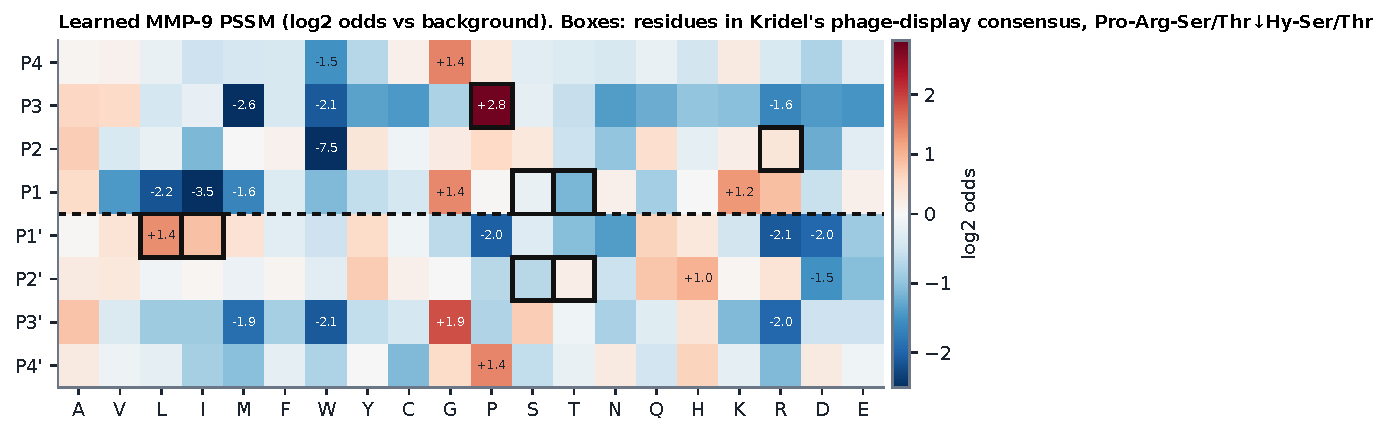
\includegraphics[width=\textwidth]{../figures/F14_mmp9_consensus.pdf}
  \caption{Learned MMP-9 PSSM (log$_2$ odds against background; cells with
    $|{\cdot}|>1$ bit are annotated). Boxes mark the residues of the Kridel et al.\
    phage-display consensus. Pro at $\pos{3}$ and Leu/Ile at $\prm{1}$ are
    recovered; Ser/Thr at $\pos{1}$ and $\prm{2}$ are not.}
  \label{fig:kcons}
\end{figure}

\subsection{Learned specificity and the enzyme structures}
\label{sec:structures}

One experimental structure per protease was prepared (table below), and
active-site facts were derived from the coordinates. In MMP-9, MMP-2 and MMP-8
the sequence around the catalytic zinc reads H-E-F-G-H-A-L-G-L-D/E-H, the
HEXXHXXGXXH motif of Nagase and Woessner \cit{2} \CONF; the zinc is coordinated
by the two histidines of HEXXH and the third histidine of the motif (His401,
His405 and His411 in MMP-9), and the hydroxamate oxygen of the bound MMP-9
inhibitor lies $2.07$~\AA\ from it \CONF. In LasB the zinc ligands are His140,
His144 and Glu164; in neutrophil elastase the catalytic triad is His57, Asp102
and Ser195 \CONF. Residues lining the ligand-occupied pocket of MMP-9 include
Asp185-Gly186-Leu187, the Asp-Gly-Leu segment that Kridel et al.\ assign to the
S2$'$ subsite (their numbering differs), and Met422. In NE they include Val190,
Ala213 and Val216, small aliphatic side chains, and the top residues of the NE
model at $\pos{1}$ are Val, Ile and Thr.

\begin{center}
\small\renewcommand{\arraystretch}{1.25}
\begin{tabular}{@{}llcclc@{}}\toprule
Protease & PDB & Resolution (\AA) & Residues & Catalytic site residues & Pocket residues \\\midrule
MMP-2 & 1QIB & 2.8 & 160 & HIS201, HIS205, HIS211 & 23 \\
MMP-8 & 1JAN & 2.5 & 164 & HIS197, HIS201, HIS207 & 21 \\
MMP-9 & 1GKC & 2.3 & 159 & HIS401, HIS405, HIS411 & 20 \\
Neutrophil elastase & 1HNE & 1.84 & 210 & ASP102, HIS57, SER195 & 22 \\
LasB & 1EZM & 1.5 & 298 & GLU164, HIS140, HIS144 & 27 \\
\bottomrule\end{tabular}

\end{center}

The table lists the structures used. Catalytic-site residues are those
coordinating the catalytic zinc (MMPs, LasB) or forming the catalytic triad
(NE); pocket residues lie within $6$~\AA\ of the bound ligand, or within
$9$~\AA\ of the catalytic zinc when no ligand is present. MMP-9 is taken from an
active catalytic-domain entry rather than the pro-form, whose prodomain occupies
the cleft \cit{10}.

\begin{figure}[H]
  \centering
  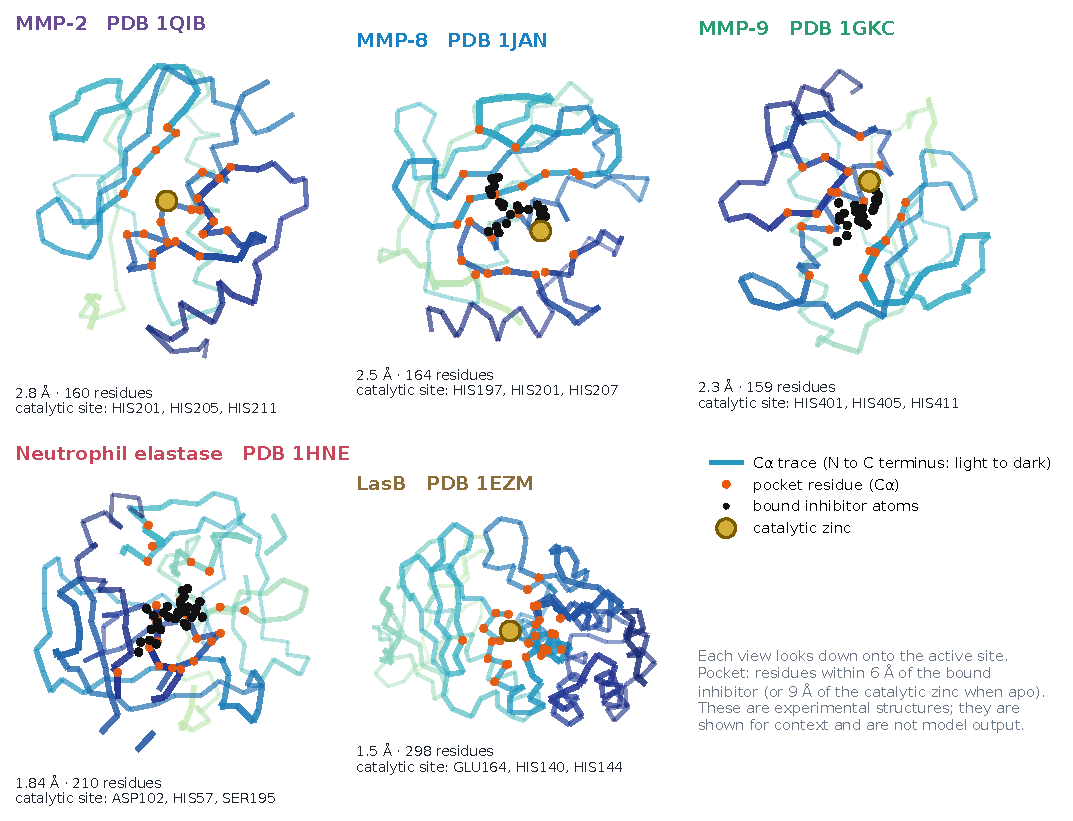
\includegraphics[width=\textwidth]{../figures/F19_structures.pdf}
  \caption{C$\alpha$ traces of the five structures, each oriented toward the
    active site (depth-cued; N to C terminus from light to dark). Orange: pocket
    residues; gold: catalytic zinc; black: bound inhibitor atoms. The structures
    are experimental and are shown for context; they are not model output.}
  \label{fig:struct}
\end{figure}

\subsection{Held-out measured kinetics}

Kridel et al.\ \cit{1} measured $\kcat/\Km$ for MMP-9 on eleven synthetic
peptides and detected no activity on a twelfth (C11). Training windows that
coincide with a validation peptide on at least seven positions (four windows)
were removed from every training set and the MMP-9 model was retrained before
scoring. Each peptide was scored as a gapped window and rank-correlated with
$\log_{10}\kcat/\Km$.

\begin{center}
\small\renewcommand{\arraystretch}{1.25}
\begin{tabular}{@{}llrrrr@{}}\toprule
Peptide & Window (P4--P4$'$) & Positions & MMP-9 $k_\mathrm{cat}/K_m$ (M$^{-1}$s$^{-1}$) & LR logit & PSSM \\\midrule
C15 & \texttt{GPRQITA-} & 7 & 188{,}000 & +2.07 & +5.41 \\
A11 & \texttt{IPRTLTA-} & 7 & 67{,}500 & +1.30 & +3.67 \\
A6 & \texttt{GPRAVSTT} & 8 & 61{,}000 & +1.24 & +4.20 \\
A11m1 & \texttt{IPRRLTA-} & 7 & 160{,}000 & +2.43 & +5.66 \\
A11m2 & \texttt{IPRTATA-} & 7 & 2{,}000 & +1.15 & +2.35 \\
A10 & \texttt{GPLFYSVT} & 8 & 25{,}600 & +0.33 & +2.70 \\
B1 & \texttt{QPHYLTTA} & 8 & 8{,}800 & +0.81 & +3.10 \\
A18 & \texttt{RPAKSTA-} & 7 & 5{,}800 & +1.28 & +4.96 \\
A7 & \texttt{--SGLKAL} & 6 & 12{,}400 & +0.77 & +3.08 \\
A19 & \texttt{GSRYLTA-} & 7 & 13{,}200 & +0.74 & +3.02 \\
A16 & \texttt{SGRRLLSR} & 8 & 1{,}200 & +0.68 & +0.78 \\
C11 & \texttt{SGRRLIHH} & 8 & not detected & +0.30 & +2.47 \\
\bottomrule\end{tabular}

\end{center}

The table lists the validation peptides as P4--P4$'$ windows with measured
$\kcat/\Km$ and the scores of the retrained model. The next table gives the
rank association; the permutation $p$-value is two-sided, intervals are
bootstrap intervals over peptides, and the last rows rank C11 below every
measured peptide.

\begin{center}
\small\renewcommand{\arraystretch}{1.25}
\begin{tabular}{@{}llccc@{}}\toprule
Score & Set & Spearman $\rho$ & 95\% bootstrap CI & Permutation $p$ \\\midrule
Logistic regression & n = 11 measured & 0.58 & [-0.23, 0.93] & 0.068 \\
Logistic regression & n = 12 (C11 ranked lowest) & 0.68 & [0.02, 0.96] & 0.017 \\
PSSM & n = 11 measured & 0.70 & [-0.00, 0.96] & 0.020 \\
PSSM & n = 12 (C11 ranked lowest) & 0.75 & [0.18, 0.93] & 0.006 \\
Standardised mean & n = 11 measured & 0.57 & [-0.21, 0.90] & 0.074 \\
Standardised mean & n = 12 (C11 ranked lowest) & 0.66 & [0.06, 0.91] & 0.021 \\
\bottomrule\end{tabular}

\end{center}

The association is positive for every scorer and set. For the PSSM,
$\rho=\rhoNElevenPSSM$ on the eleven measured peptides (permutation
$p=\rhoPNElevenPSSM$; $95\%$ interval $[\rhoLoNElevenPSSM,\rhoHiNElevenPSSM]$);
for the logistic regression $\rho=\rhoNElevenLR$ ($p=\rhoPNElevenLR$). The
intervals are wide and, for the logistic regression on $n=11$, include zero.
With $n=11$ and a set that was itself selected for high activity, this is
evidence of a positive association and not of accurate rate prediction, and the
six tests are not corrected for multiplicity. By the logistic regression the
three highest-scored peptides (A11m1, C15, A11) are the three most active; its
largest miss is A10 ($25{,}600$~M$^{-1}$s$^{-1}$, the fifth most active), which it
scores second-lowest. The PSSM scores the least active measured peptide (A16)
lowest but ranks A18 ($5{,}800$) third, its largest miss.

\begin{figure}[H]
  \centering
  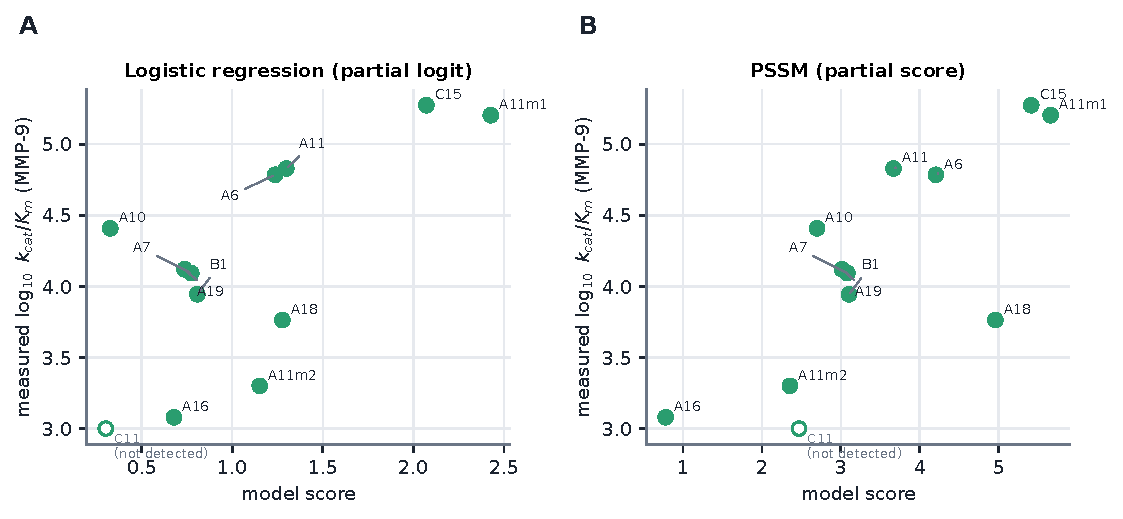
\includegraphics[width=\textwidth]{../figures/F15_kridel_validation.pdf}
  \caption{Model score against measured MMP-9 $\log_{10}\kcat/\Km$. Open marker:
    C11, no activity detected (plotted at the floor of the axis).}
  \label{fig:kval}
\end{figure}

\subsection{Matched point mutants}

Two peptides are single-substitution mutants of A11 (SGKIPRT$\downarrow$LTA):
A11m1 replaces Thr with Arg at $\pos{1}$; A11m2 replaces Leu with Ala at
$\prm{1}$. Because the background is identical, each isolates one substitution.

\begin{center}
\small\renewcommand{\arraystretch}{1.25}
\begin{tabular}{@{}llccc@{}}\toprule
Pair & Substitution & Measured fold change (log$_2$) & LR $\Delta$ (bits) & PSSM $\Delta$ (bits) \\\midrule
A11$\to$A11m1 & T7R at P1 (Thr to Arg) & 2.37$\times$ (+1.25) & +1.63 & +1.99 \\
A11$\to$A11m2 & L8A at P1' (Leu to Ala) & 0.03$\times$ (-5.08) & -0.21 & -1.31 \\
\bottomrule\end{tabular}

\end{center}

The model predicts the correct direction for both and approximately the correct
size for the first ($+\mutOneLR$ bits from the logistic regression and
$+\mutOnePSSM$ from the PSSM, against a measured $+\mutOneMeasured$ log$_2$
units). For the second it predicts a decrease but underestimates it:
$\mutTwoLR$ bits (logistic regression) and $\mutTwoPSSM$ bits (PSSM) against a
measured $\mutTwoMeasured$. Large kinetic effects of a single key residue are
compressed by a model trained to distinguish cleaved from uncleaved sites, not
fast from slow \CONF.
